\documentclass[11pt]{article}

% ========== Packages ==========
\usepackage[scaled]{helvet} % Load the helvet package to get Helvetica (similar to Nimbus Sans)
\usepackage[T1]{fontenc} % Ensures proper font encoding
\usepackage[utf8]{inputenc} % Encoding
\usepackage{graphicx} % For including images
\usepackage{amsmath, amssymb} % For mathematical symbols and equations
\usepackage{hyperref} % For hyperlinks
\usepackage{ragged2e} % Enhanced Justification and hyphenation
\usepackage[backend=biber, style=apa]{biblatex} % For the bibliography
\usepackage{geometry} % To set the margins
\usepackage{tocloft} % Customization of the Table of Contents
\usepackage{tikz} % For Drawing Diagrams
\usepackage{float} % Better control over placement of figures and tables


% ========== PREAMBLE ==========

% ********** Macros **********
\newcommand{\needcite}{\textbf{\color{red}[CITATION NEEDED]}}
\newcommand{\needs}[1]{\textbf{\color{red}[\MakeUppercase{#1}]}}

% ********** Package Setups **********
\addbibresource{references.bib} % The filename of your bibliography file
\usetikzlibrary{shapes, arrows.meta, positioning, calc}

% ********** Formatting **********
\linespread{1.2}% Set line spacing to ~1.5
\setlength{\parindent}{0pt} % No indentation at the beginning of paragraphs
\setlength{\parskip}{1em} % Adds vertical space between paragraphs
\renewcommand*\familydefault{\sfdefault} % Set the default font to the sans-serif font
\setlength{\cftbeforesecskip}{5pt} % Set space before each ToC section entry to 0pt
\geometry{
  top=1in,    % Top margin
  bottom=1in, % Bottom margin
  left=1in,   % Left margin
  right=1in   % Right margin
}
\hypersetup{
    colorlinks = true, % Colored links instead of boxed
    linkcolor = blue, % Color of internal links
    citecolor = blue, % Color of citations
    urlcolor = blue, % Color of URLs
    pdfborder = {0 0 0}, % Remove border around links
    linktocpage = true, % Makes the page number the link in the ToC
    pdfnewwindow = true, % Links in new PDF window
    pdfstartview = {FitH}, % Fits the width of the page to the window
    pdftitle = {W3.io Whitepaper}, % Title
    pdfauthor = {Audie Sheridan, Ben Murray, David Post}, % Author
    pdfsubject = {Blockchain Integration Solutions}, % Subject
    pdfkeywords = {blockchain, decentralized, web3}, % Keywords
}

% ********** Hyphenation Rules **********
\hyphenation{block-chain}

% ********** REMOVE IN FINISHED VERSION **********
% Write DRAFT angled over every page
\AddToHook{shipout/background}{%
  \put(0,0){%
    \begin{tikzpicture}[remember picture,overlay]
      \node[opacity=0.3, scale=15, rotate=45] at (current page.center) {DRAFT};
    \end{tikzpicture}%
  }
}

% ========== BEGIN DOCUMENT ==========

\begin{document}

% ********** Title Page **********

\begin{titlepage}
    \centering
    \vspace*{1cm} % Adjust the vertical space as needed
    
\includegraphics[width=0.4\textwidth]{images/w3io-logo-vertical-positive.png} % Adjust the path and width as needed
    
    \vspace{0.5cm}
    {\large \textbf{Bridging Blockchain and Off-Chain Compute}\par}
    \vspace{0.5cm}
    {\large \textbf{Making Hard Things Easy In Web3}\par}
    \vspace{0.5cm}
    {\large Version 0.1\par}
    \vspace{4cm}
    {\large Audie Sheridan, Ben Murray, David Post\par}
    \vfill
    {\large \today\par}
\end{titlepage}

% ********** Table of Contents **********

\newpage
\tableofcontents % This line adds the Table of Contents
\newpage

% ********** Abstract **********

% temporary hyphen rules for the abstract
\hyphenpenalty=5000
\exhyphenpenalty=5000
\begin{abstract}
\justifying % Full Justification for the abstract
\noindent
W3.io introduces a protocol aimed at bridging the gap between blockchain's on-chain execution capabilities and the computational power of the many decentralized off-chain compute projects in web3. This integration tackles real-world business challenges by enabling seamless orchestration of diverse on and off-chain compute tasks across a network of decentralized nodes. Despite the proliferation of decentralized solutions addressing various computational needs, a significant gap remains in integrating these solutions to address complex business processes effectively. W3.io proposes a decentralized network where nodes are incentivized to execute compute tasks, acting as the glue that integrates on-chain and off-chain computations. Through customizable recipes and ingredients, users can define and execute business processes with unprecedented flexibility and efficiency. The initiative is poised to redefine how businesses interact with blockchain ecosystems, offering a more integrated, efficient, and scalable approach to solving real-world problems. This enhances the capabilities of existing decentralized applications and opens new avenues for innovation and collaboration within the web3 space.
\end{abstract}
\hyphenpenalty=50 % Resetting to default values 
\exhyphenpenalty=50
\newpage

% ********** Main Document **********

\section{Introduction}
Blockchain tech is a revolution in how we handle digital transactions and build decentralized apps, promising security and transparency. But it's not a magic bullet—it's got its limits. Things like slow transaction speeds, high costs, and limited on-chain power mean it can't do everything on its own, so we take much of the work off-chain. In the past few years, many decentralized projects launched that can replace small parts of IT offers with more efficient decentralized options. 

There is a proliferation in individual chains. Some projects strive to be cross chain, others launch their own special purpose chains. It's become difficult to keep up, and the immense value web3 off-chain compute projects bring remains hidden and difficult to access. Web3 is both difficult and vast. 

W3.io emerges as a pioneering solution in this landscape, designed to bridge the gap between the on-chain capabilities of blockchain technologies and the computational power of off-chain systems. This whitepaper introduces the W3.io protocol, a decentralized framework that facilitates seamless orchestration of on-chain and off-chain compute tasks. By leveraging a network of decentralized nodes, W3.io enables businesses to execute complex, integrated workflows with enhanced efficiency and flexibility.

The need for such a solution is driven by several critical challenges currently faced by developers and enterprises in the web3 space. Firstly, the over-reliance on centralized services contradicts the decentralized ethos of blockchain, introducing risks such as single points of failure and potential censorship. Secondly, the technical complexities involved in integrating disparate IT systems can stifle innovation and escalate costs. Lastly, the business challenges of deploying decentralized solutions—such as legal intricacies, payment issues, and the steep learning curve associated with new technologies—can deter enterprises from adopting blockchain technology.

W3.io addresses these challenges by providing a decentralized network of nodes that acts as an integrative backbone for . The protocol supports customizable "recipes" that define workflows triggered by user-defined events, progressing through a series of verifiable operations executed by the network nodes. This approach not only democratizes access to blockchain technology but also enhances the operational capabilities of existing decentralized applications, paving the way for innovative, complex, decentralized solutions.

This whitepaper details the architecture, operation, and potential applications of the W3.io network, illustrating how it can transform the landscape of blockchain integration and foster a new wave of decentralized innovation. By reducing dependency on centralized infrastructures, simplifying integration challenges, and addressing key business hurdles, W3.io is poised to play a crucial role in the evolution of blockchain ecosystems.

\section{Problem Statement}
When grappling with the world of web3, developers and businesses face a trio of challenges that can often slip under the radar in the rush to innovate. These hurdles include a heavy reliance on centralized services, the technical headaches of integration, and the business complexities of deploying complex decentralized solutions.

\subsection{Dependence on Centralized Services}
On the business front, the main priority often boils down to speed of delivery \parencite{elliot2014devops}, which naturally pushes developers towards the ready-to-go, easy-to-use centralized solutions. This not only shifts on-chain value off-chain but also racks up about \$180 million annually spent by web3 projects on centralized compute.\needcite The convenience of centralized compute services like Amazon Web Services, Google Cloud, and Microsoft Azure is undeniable. They make spinning up new servers, containers or functions a breeze, which is why they're so attractive to web3 developers. However, this reliance is at odds with the decentralized ethos of web3 and brings with it several significant drawbacks:
\begin{itemize}
  \item \textbf{Centralization Risks:} Using centralized services introduces single points of failure and potential censorship or control by central authorities, which goes against the grain of web3's decentralized promise. \parencite{nakamoto2008bitcoin}
  \item \textbf{Data Privacy Concerns:} There's always a risk that data processed on centralized platforms could be accessed or misused, posing serious privacy risks for sensitive blockchain applications. \parencite{zyskind2015decentralizing}
  \item \textbf{Vendor Lock-in:} Being tied to specific cloud providers can lead to vendor lock-in, making it tough and expensive to switch services or operate in a truly decentralized fashion. \parencite{armbrust2010view}
  \item \textbf{Cost Predictability:} The costs of using centralized compute services can be unpredictable and may spiral as operations grow, which is a challenge for projects on tight budgets. \parencite{vaquero2014finding}
  \item \textbf{Network Latency:} Relying on centralized servers can introduce latency issues, especially when the blockchain network is spread worldwide but the compute resources are centralized in specific locations. \parencite{bonomi2012fog}
  \item \textbf{Regulatory Exposure:} Centralized services are subject to the laws and regulations of the places they operate in, which can bring additional constraints and risks not present in a decentralized setup. \parencite[see Chapters 7 and 10]{lessig1999code}
\end{itemize}

\subsection{Technical Difficulties}
Piecing together various parts of the IT stack in a decentralized way to solve a complex business problem is currently quite a challenge. Starting such an integration requires not only hiring pricey web3 development talent but often also involves that talent firing up centralized compute to build and test everything piece by disconnected piece. The lack of a common agreement on which blockchain to use only adds to the testing and development problems. Different decentralized solution providers may have dramatically different ways of working with blockchain technology. 

Developers working in web3 often find themselves doing tedious tasks during integration type projects. Things like translating data, simple data storage, devops, IT administration, and any other of a host of things required to make the customer project work, but that they've also done a hundred times before. Most web3 development is bespoke, and consists of easily repeatable patterns. This presents multiple risks for the customers:
\begin{itemize}
  \item \textbf{High Development Costs:} Web3 development is obscenely expensive, and you don't pay less for hours spent solving tedious work orthogonal to the crux of your business problem.
  \item \textbf{Suboptimal Integrations:} Developers hired by you to develop your solutions will not be expert on every integration you need, so the quality of those integrations will vary widely
  \item \textbf{Chance of Failure:} Software development projects often fail, and complexity multiplies the chances of that. The less code you need to solve your business problem, the better.
  \item \textbf{Brittle Solutions:} Your solution may ultimately succeed, but a bespoke implementation will require specialized maintenance. The availability of your developer in a year or two, when the solution needs an upgrade or bug fix, is uncertain. Reliability in a crisis is also not guaranteed.
\end{itemize}

\subsection{Business Challenges}
The task of using multiple decentralized services together to tackle business needs isn't just technically demanding—it's also time-consuming and costly. In order to use multiple off-chain computation providers to solve your business problems, you have to know them well. You have to be technically competent about their solution and how to use it, you have to arrange terms, engage legal services perhaps, and most importantly, perhaps, you have to \textit{wait} until these challenges are finished to launch the actual solution you're after. 

In addition to the hurdles in place if you already know the decentralized solution providers you want to use, there is the problem of even being aware a solution you could use exists. There are hundreds or thousands of decentralized projects, each with their own unique perspective. They vary in how well they tell you \textit{what} they do and \textit{how} they do it, but most are bad at describing \textit{why} you should be interested. Just knowing the possibilities presents its own challenge. 

Assuming a customer were able to navigate all the above business challenges, then comes the problem of payment. With a multitude of partners, chains, and other providers, coordinating proper payment will be a significant barrier. Some providers will want payment at time of service, others as a subscription (overbuying for your need), blockchains require gas or fees to execute, partner payments might require holding tokens or just paying in specific tokens. All of this adds up to a significant headache for even a slightly complex business process.  

\section{W3.io Solution}
W3.io directly addresses the trio of challenges identified in the Problem Statement—dependence on centralized services, technical integration difficulties, and complex business deployments—by establishing a decentralized network that acts as the integrative backbone for various IT verticalsa and other solutions provided by our network partners. This network not only supports blockchain operations but also seamlessly ties together services from over 40 decentralized compute partners, making it a robust solution for real-world business applications.
\begin{itemize}
    \item \textbf{Decentralized Network as a Solution to Centralization:} Our decentralized network mitigates the risks associated with centralization, such as single points of failure and potential censorship, by distributing compute tasks across an array of decentralized nodes. This structure ensures enhanced data privacy and reduces regulatory exposure, aligning with the decentralized ethos of web3 and improving cost predictability.
    \item \textbf{Integration of Decentralized Compute Partners:} The core of W3.io's functionality lies in its ability to orchestrate complex compute tasks through customizable 'recipes.' These recipes define workflows that begin with a customer-defined trigger and progresses through a series of decentralized operations. Each step in a recipe is executed verifiably by either a decentralized compute partner, or by the node in w3.io that interacts with the blockchain or external provider needed. This ensures the integration of multiple decentralized partners is seamless and efficient.
    \item \textbf{Addressing Technical and Business Challenges:} By leveraging the specialized capabilities of our decentralized partners, W3.io addresses the high costs and technical challenges associated with web3 development. Each partner can act as an 'ingredient' in our recipes, allowing us to provide a broad IT solution that is both repeatable and testable. This approach significantly reduces the redundancy and inefficiency typically involved in bespoke web3 projects, thereby lowering development costs and enhancing project viability.
    \item \textbf{Pre-built Network for Rapid Deployment:} W3.io has pre-established agreements with a diverse range of decentralized compute partners, enabling rapid deployment of decentralized solutions. This ready-to-deploy framework is crucial for businesses looking to integrate complex systems without the need for extensive legal or technical groundwork. Our model simplifies the process of using multiple decentralized services, thereby solving the business challenge of lengthy and costly integrations.
    \item \textbf{Unified Payments:} Due to the established agreements with the decentralized compute partners, w3.io will consolidate the payment needed for these partners. Instead of separately paying several partners, any involved chain's fees, or other integrated provider, w3.io will provide the option of paying once for the entire workflow. This will provide a means to abstract the payment from the underlying complexity, which w3.io will navigate on behalf of the customer.
\end{itemize}

W3.io provides a comprehensive solution that not only addresses the inherent challenges of web3 development but also enhances the capabilities of blockchain technology by making it easy to integrate it with off-chain compute resources. Through our network of decentralized partners and our decentralized node network running customizable recipes, we offer businesses a scalable, efficient, and secure platform to execute their operations, paving the way for innovative applications in the web3 space.

\section{Ecosystem and Partnerships}
\needs{NEEDS DAVID AND BEN COPYWRITING AND EDITING}

One of the most important aspects of how W3.io builds value is in the strength of the network of decentralized compute providers and chains that want to be a part of this solution. The effort to assemble over 40 partners into this network was a massive, 2 year undertaking, and reflects our commitment to a broad and effective ecosystem.

\subsection{Building a Strong Network}
The establishment of our partner network is not just about quantity but also about the quality and synergy between the partners. Each partner has been carefully selected based on their commitment to the vision of decentralized solutions and their ability to solve specific business problems. This pre-established network not only saves our customers the effort of vetting potential service providers but also ensures that they have access to top-tier solutions across the blockchain and IT spectrum.

\subsection{Knowledge and Integration}
We understand our partners' capabilities deeply and bring this knowledge to bear for the benefit of our customers. By building integrations in cooperation with our partners, we ensure that these integrations are robust, effective, and tailored to real-world applications. This collaborative approach enhances the functionality and reliability of our ecosystem, providing our customers with seamless access to a comprehensive suite of services.

\subsection{Transparency and Accessibility}
In our network, each partner is exposed in a way that highlights their strengths and unique offerings. We make it clear why customers should choose these solutions, aiding in informed decision-making. Importantly, W3.io is not rent-extractive towards our partners; we do not charge them for participation in our network. Instead, our model is designed to benefit our partners by exposing them to a broader customer base, thereby enhancing their business development opportunities.

\subsection{Synergistic Benefits}
The collaborative environment of our network means that every partner's business development efforts indirectly benefit all other partners. Since each partner typically offers only a part of the complete IT/Blockchain solution a customer might need, our platform facilitates the integration of these various services into cohesive solutions. This is achieved without the need for complex business agreements directly between multiple partners, as W3.io provides a unified framework with rules that are flexible enough to accommodate diverse solutions yet strict enough to ensure effective problem-solving.

\subsection{Conclusion}
The ecosystem of partners within W3.io is a cornerstone of our strategy to provide decentralized, integrated solutions that are more than the sum of their parts. By fostering a network where collaboration and mutual benefit are key, we not only enhance the capabilities of individual partners but also create a more robust and versatile platform for our customers. This network-driven approach is pivotal in redefining how businesses interact with blockchain technologies and decentralized applications, paving the way for innovative solutions in the web3 space. 


\section{Partner Usage In Protocol}
In the development and operation of the W3.io protocol, the integration of our partners' solutions is not just a feature---it's a fundamental aspect of our architecture. By incorporating our partners directly into the core of our protocol, we demonstrate the same trust and reliance on decentralized solutions that we advocate to our customers. This approach not only enhances the robustness and capabilities of the W3.io network but also serves as a live case study for the potential and effectiveness of decentralized compute resources.

\subsubsection*{Strategic Integration of Partners}
Our protocol leverages the specialized services offered by our partners to address internal operational needs, mirroring the integration challenges our customers face. This strategic use of partners' technologies within our core operations serves multiple purposes:
\begin{itemize}
    \item \textbf{Proof of Concept}: By using our partners' solutions to solve our own challenges, we provide a tangible proof of concept that showcases the practical applications and benefits of these technologies. This not only builds confidence in our protocol but also demonstrates the real-world utility of our partners' offerings.
    \item \textbf{Enhanced Credibility}: Integrating our partners deeply into our protocol operations enhances the credibility of our network. It shows that we stand behind the decentralized ethos we promote, committing to the same solutions we recommend to our users.
    \item \textbf{Continuous Improvement and Feedback}: This close integration allows us to continuously test, evaluate, and provide feedback on the technologies we use. It creates a feedback loop that benefits both W3.io and our partners, leading to improvements and optimizations in the solutions offered.
\end{itemize}

\subsubsection*{Transparency and Choice}
Transparency is key in decentralized systems, and at W3.io, we commit to maintaining a high level of transparency regarding which partners we integrate and why. By publishing our choices and the rationale behind them, we aim to:
\begin{itemize}
    \item \textbf{Educate Our Users}: Help our users understand why certain decentralized solutions are chosen over others and how they can be leveraged effectively in different scenarios.
    \item \textbf{Promote Informed Decision-Making}: By sharing our experiences and insights, we enable our customers to make informed decisions about which technologies and partners might best meet their own needs.
    \item \textbf{Foster a Collaborative Ecosystem}: Transparency about our use of partners' solutions encourages a collaborative environment where knowledge and best practices are shared, benefiting the entire ecosystem.
\end{itemize}

\subsubsection*{Benefits of Partner Integration}
Integrating our partners into the core of our protocol offers several benefits:
\begin{itemize}
    \item \textbf{Reliability and Security}: Using proven decentralized solutions enhances the reliability and security of our network, aligning with our goal to reduce reliance on centralized systems.
    \item \textbf{Scalability}: Leveraging partners' technologies allows us to scale more efficiently by utilizing their expertise and solutions to handle specific tasks or challenges.
    \item \textbf{Innovation}: This approach fosters innovation by encouraging the use of cutting-edge technologies and solutions that may not be available in traditional systems.
\end{itemize}

The strategic integration of our partners into the W3.io protocol is a deliberate choice that underscores our commitment to the decentralized model. It not only enhances our protocol's functionality and reliability but also sets a standard for transparency and collaboration in the web3 space. By doing so, we not only advocate for the adoption of decentralized solutions but also \textit{lead by example}, showcasing the practical benefits and operational enhancements these technologies bring to the table. 

\section{User Experience (UX)}
At W3.io, we simplify the complex landscape of web3 with a user experience designed to make hard things easy. Our interfaces guide both technical and non-technical users through the intricacies of blockchain technology, providing clear, actionable tools and resources. This approach not only exposes and demystifies potential dangers but also empowers our partners and customers to focus on solving their business challenges effectively. For developers, we streamline the foundational aspects of web3 development, allowing them to concentrate on creating innovative solutions rather than getting bogged down by routine tasks. The UI showcases how and why to use the tools and services offered by our partners, making it clear how each partner contributes to solving specific business problems. This visibility fosters an environment of innovation, where Customers and their developers are freed from the minutiae to focus on crafting new and unique solutions.
 
\needs{DIAGRAM OF ON AND OFF-CHAIN COMPUTE INTEGRATION}

\subsection{CLI}
The Command Line Interface (CLI) provides power users with the ability to interact directly with the W3.io protocol through command-line tools. This interface is ideal for automation and scripting tasks.

\subsection{Visual}
The visual interface of W3.io is structured to facilitate the creation and management of recipes and ingredients, which are central to representing business problems within the w3.io protocol. This interface visually maps out the flow of operations, where each step or box in the flow chart represents an interaction with partners, blockchain technologies, or the recipe's data. This approach simplifies complex processes into manageable components, making it intuitive for users to design and oversee their business solutions.

\section{Ingredients}
Ingredients are the fundamental building blocks within the W3.io ecosystem, representing specific tasks or operations executable as part of a recipe. These modular and reusable components can execute functions such as accessing databases, performing calculations, or interacting with blockchains. They can add or modify variables within the recipe's variable pool to maintain state throughout execution and generate verifiable logs for integrity and traceability.

Ingredients can be simple, performing a single task, or compound, consisting of multiple sub-ingredients for more complex operations. This design enhances flexibility and scalability in developing business solutions.

A special type of Ingredient called a "Trigger" is the entry point to a recipe. Every business process can be consider a reaction to something, whether that is a schedule elapsing, an email receipt, an api call, or a blockchain event occurring. Anything like this can be built into a trigger, and when the trigger occurs, the recipe will run against the specific information from that trigger. 

Partners will work with w3.io and other partners to ensure the ingredients integrate their tools well. Where partners naturally solve a more complex problem together, they can create and publish compound ingredients to the benefit of all involved. An example of that is below: 

\begin{figure}[H]
  \centering
  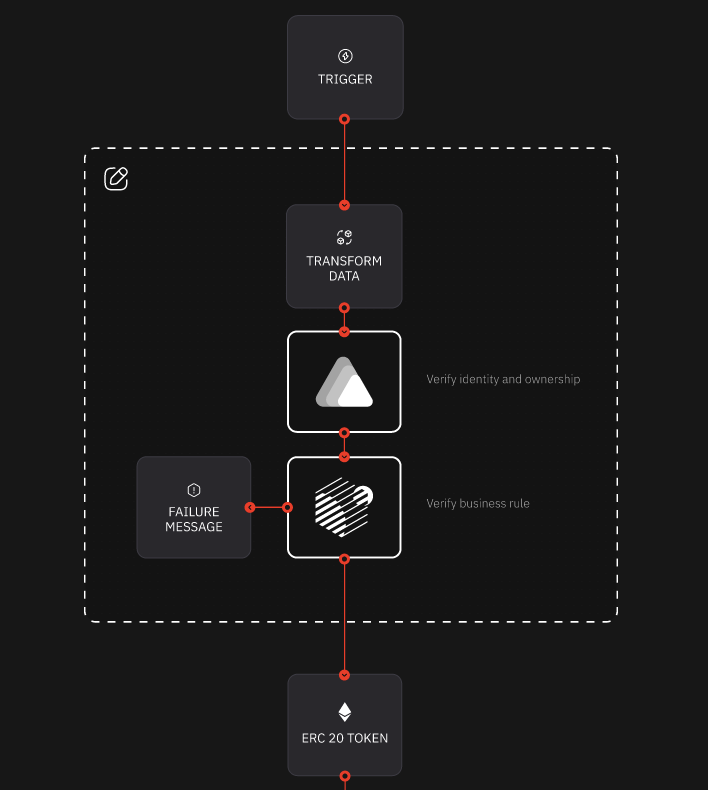
\includegraphics[width=0.40\textwidth]{images/Compound Ingredient.png}
  \caption{Illustration of a Compound Ingredient in W3.io}
  \label{fig:compoundingredient}
\end{figure}

\section{Recipes}
Recipes in W3.io are structured workflows composed of multiple ingredients, defining complete business processes triggered by specific events. These can be consider the template for what should be done given a specific event defined by the trigger. When the trigger fires and the recipe begins to run, it's then running against specific conditions. 

Each recipe includes:
\begin{itemize}
    \item \textbf{Trigger}: Initiates execution, triggered by events such as a time-based event, a transaction on a blockchain, or an external API call.
    \item \textbf{Variable Pool}: Provides dynamic data storage, enabling ingredients to share and modify data throughout the recipe's execution.
    \item \textbf{Workflow Steps}: Ordered sequence where each ingredient processes data and passes results to the next step.
    \item \textbf{Failure Handling}: Mechanisms to manage errors or exceptions, including logging errors, retrying steps, or executing alternative workflows.
\end{itemize}

\begin{figure}[H]
    \centering
    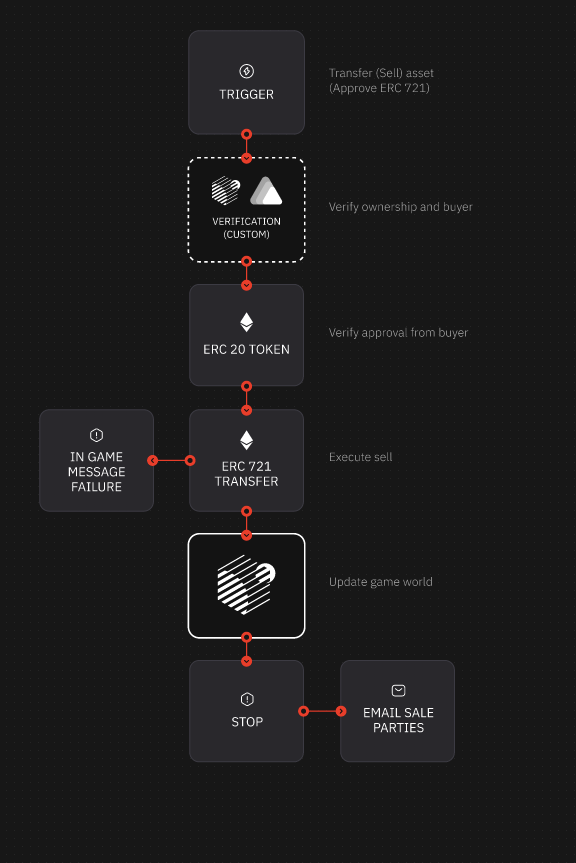
\includegraphics[width=0.40\textwidth]{images/Recipe.png}
    \caption{Illustration of a Typical Recipe Workflow in W3.io}
    \label{fig:recipe}
\end{figure}

Recipes are highly customizable and adaptable to a wide range of business needs, making them a powerful tool for integrating decentralized computing resources into coherent, executable workflows.

\paragraph{Deployment}
Once a recipe design is complete, then the customer would arrange payment for when the recipe runs, and then deploy the recipe into the w3.io protocol. Deployment tools within the visual interface allow users to easily deploy their recipes into the decentralized network, ensuring that their business processes are executed as designed. 

\paragraph{Payment}
The payment interface simplifies the process of handling transactions within the W3.io network. It provides a unified method for managing payments for services rendered by various decentralized compute partners.

\section{W3.io Protocol}
The W3.io protocol serves as the foundational framework of the network, enabling the seamless integration of decentralized computing resources and blockchain technologies. At the heart of W3.io is an incentivized network of nodes, each contributing computing power to the collective network. These nodes engage in a decentralized task queue that tracks and manages the execution of recipes and their constituent ingredients (or tasks). All nodes operate on a uniform core code, structured as a finite state machine, which collaborates across the network to achieve the necessary consensus for each recipe. Unlike traditional blockchain systems, these nodes operate at their native compute speeds, functioning purely as a distributed network of computers sharing computational resources. The next sections will get deeper into the network structure, node functionalities, and the decentralized task queue, providing a comprehensive understanding of the W3.io protocol's operational dynamics.

\subsection{Network}

\begin{figure}[H]
    \centering
    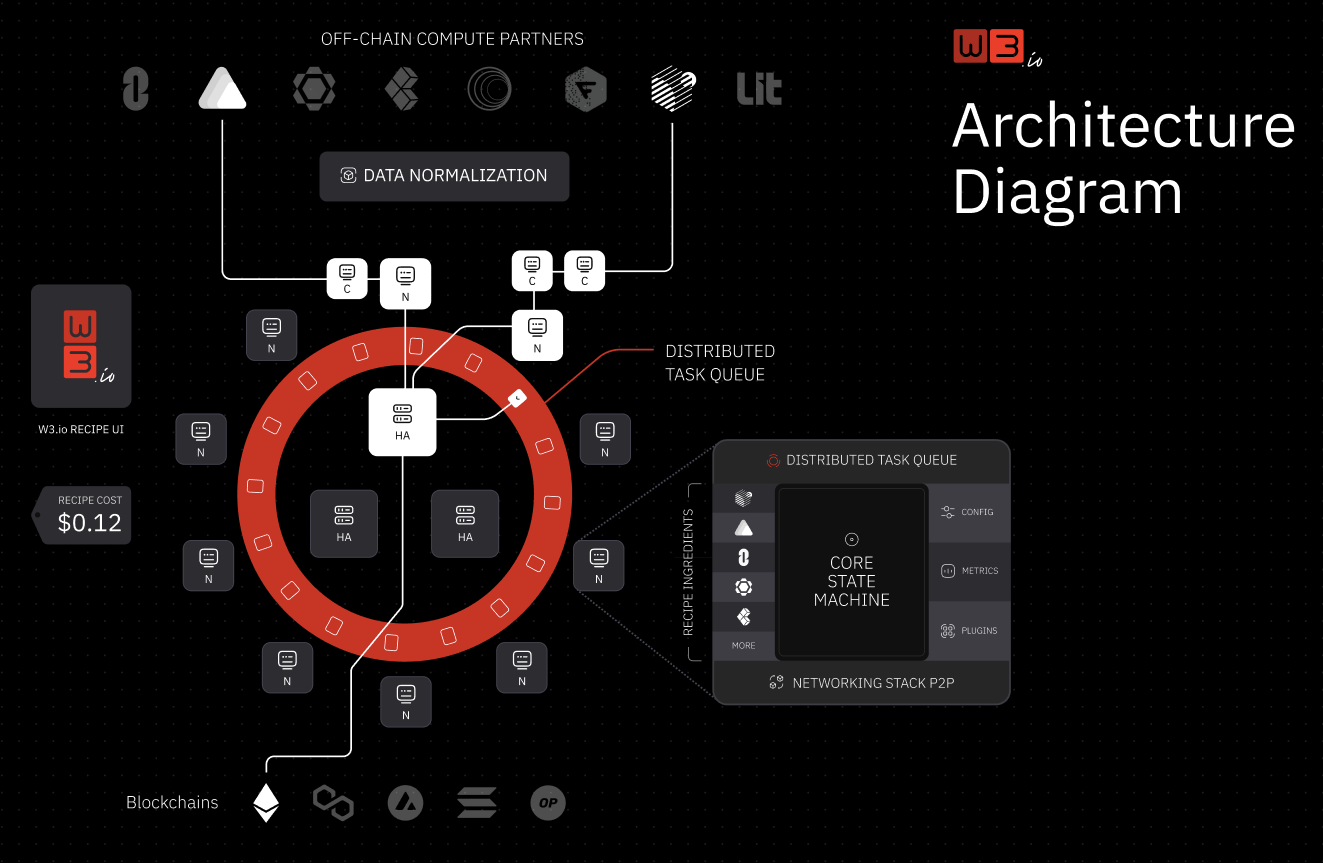
\includegraphics[width=\textwidth]{images/Architecture Diagram.png}
    \caption{Architecture Overview of the W3.io Network}
    \label{fig:network}
\end{figure}

\subsection{Nodes}
Nodes are the operational units within the W3.io network, each contributing essential computing power to facilitate the execution of decentralized tasks. These nodes are incentivized to participate actively in the network, ensuring that customer-defined business processes are executed efficiently and reliably.

\begin{figure}[H]
  \centering
  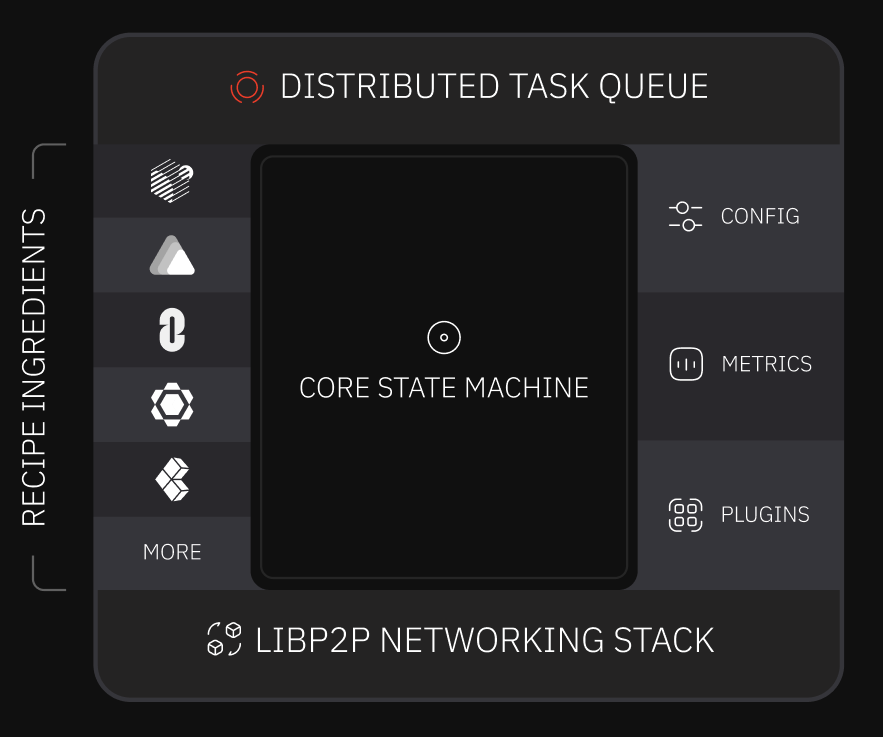
\includegraphics[width=0.5\textwidth]{images/Node.png}
  \caption{Node Architecture}
  \label{fig:node architecture}
\end{figure}

Each node within the network operates based on a uniform core code, which functions as an event-driven finite state machine. This design is optimized to minimize the computational overhead not directly related to customer recipes, thereby enhancing the overall efficiency of the network.

The choice of programming language for implementing the nodes in the W3.io network was a critical decision influenced by several factors that prioritize safety, performance, and reliability. After careful consideration, Rust was selected as the primary language for node development. Rust provides several advantages that align well with the needs of a decentralized compute network like W3.io.

\begin{itemize}
    \item \textbf{Memory Safety:} Rust's ownership model ensures memory safety without the overhead of garbage collection, which is crucial for maintaining high performance and avoiding common security vulnerabilities like buffer overflows \parencite{matsakis2014rust}.
    \item \textbf{Concurrency:} Rust's approach to concurrency is based on the concept of 'fearless concurrency', which allows developers to write code that is free from data races and other concurrency issues, making it ideal for the distributed nature of the nodes \parencite{levy2015ownership}.
    \item \textbf{Performance:} Rust offers performance comparable to C and C++, which is essential for the compute-intensive tasks that nodes must handle in the W3.io network \parencite{anderson2016rust}.
    \item \textbf{Robust Ecosystem:} Rust's growing ecosystem of libraries and tools, particularly for network programming and cryptography, provides a strong foundation for developing secure and efficient node software \parencite{blandy2017programming}.
\end{itemize}

\subsubsection*{Core Components of a Node}
\begin{itemize}
    \item \textbf{LibP2P Networking Stack:} Each node is equipped with a LibP2P networking stack, which forms the backbone of node-to-node communication. This stack facilitates a robust and decentralized connectivity framework, allowing nodes to interact seamlessly across the network.
    
    \item \textbf{Core State Machine:} At the heart of each node is a core state machine that manages the node's operations based on incoming events. This state machine ensures that each node responds appropriately to changes in network conditions or task requirements.
    
    \item \textbf{Configuration System:} Nodes feature a flexible configuration system tailored to the hardware specifications on which they operate. This system allows nodes to optimize their performance and resource utilization effectively.
    
    \item \textbf{Metrics System:} A built-in metrics system enables the monitoring of each node’s performance and participation in the network. This system is crucial for maintaining operational transparency and for the continuous improvement of node efficiency.
    
    \item \textbf{Plugins:} Nodes can be extended with various plugins that utilize the underlying hardware resources or add new functionalities. For example, a plugin might enable a node to register itself in a specific geographical locale or enhance its computational capabilities.
    
    \item \textbf{Recipe Ingredients:} Each node stores and manages the ingredients required to execute the recipes. These ingredients are modular components that nodes combine to perform complex business processes as defined in the recipes.
    
    \item \textbf{Distributed Task Queue:} Nodes participate in a distributed task queue, a crucial component that assigns tasks to nodes based on their availability and capability. This queue ensures that tasks are distributed efficiently across the network, minimizing delays and optimizing resource use.
\end{itemize}

These components collectively ensure that each node within the W3.io network can operate autonomously yet cohesively, contributing to the network's goal of providing a decentralized, efficient, and reliable platform for executing complex business workflows.


\subsection{Types of Nodes}
The W3.io network accommodates diverse computing resources by categorizing nodes into three types: High Availability Nodes, Normal Nodes, and Community Nodes. This classification is designed to maximize compute participation across different hardware capabilities and availability.

\subsubsection{High Availability Nodes}
High Availability Nodes are designed to offer robust services with a target of 99.999\% uptime, often referred to as "five nines" availability. These nodes are typically equipped with advanced compute resources such as Trusted Execution Environments (TEEs), GPUs, substantial disk space, and high-performance CPUs. They are incentivized to maintain high availability and performance, playing a crucial role in handling critical tasks within the network.

\subsubsection{Normal Nodes}
Normal Nodes are akin to desktop computers in residential settings. They are expected to be online consistently, though they may occasionally face connectivity or power interruptions. These nodes form the backbone of the network, ensuring widespread participation and resource availability.

\subsubsection{Community Nodes}
Community Nodes include devices with intermittent connectivity and availability, such as laptops and smartphones. Users can connect these devices to the network during periods of non-use, such as overnight, to contribute resources while earning compute incentives. This category allows for casual participation from a broad user base, enhancing the network's decentralization.

\paragraph{Network Participation}
All nodes, regardless of their category, participate as consensus peers within the network. They execute tasks, or "ingredients," assigned to them, contributing to the network's overall computational power and reliability. Unlike the Internet Computer Protocol (ICP) by Dfinity, where providing compute resources can be a costly investment, W3.io aims to lower the barriers to entry. This approach allows individuals to contribute to the network with existing devices, reducing the need for specialized hardware and significant upfront costs. This model contrasts sharply with ICP's infrastructure requirements, making W3.io more accessible to a broader audience \parencite{dfinity2018overview}.


\subsubsection{Compute Execution}
Nodes handle various compute tasks, categorized into customer compute and protocol compute.

\paragraph{Customer Compute}
Customer compute tasks are initiated by external triggers. Nodes listen for these triggers and execute the corresponding recipes.

\paragraph{Protocol Compute}
Protocol compute tasks are internal operations necessary for the maintenance and operation of the W3.io network.

\subsubsection{Verifiability}
Verifiability in the W3.io network begins at the moment an operation is triggered. Multiple nodes may listen for and "hear" this trigger, which could originate from various sources such as API calls, scheduled events, or blockchain transactions. Upon detection, the data is immediately subjected to a verification process using a customer-defined consensus mechanism. This ensures the authenticity and correctness of the data before any further processing.

Once verified, the context—which includes details about the executing nodes, the incoming data, and recipe metadata—is recorded in an ephemeral log. This log entry is then hashed, and the resulting hash is passed along to the next step in the recipe execution process. This procedure of logging and hashing continues throughout the execution of the recipe.

\begin{figure}[H]
  \centering
  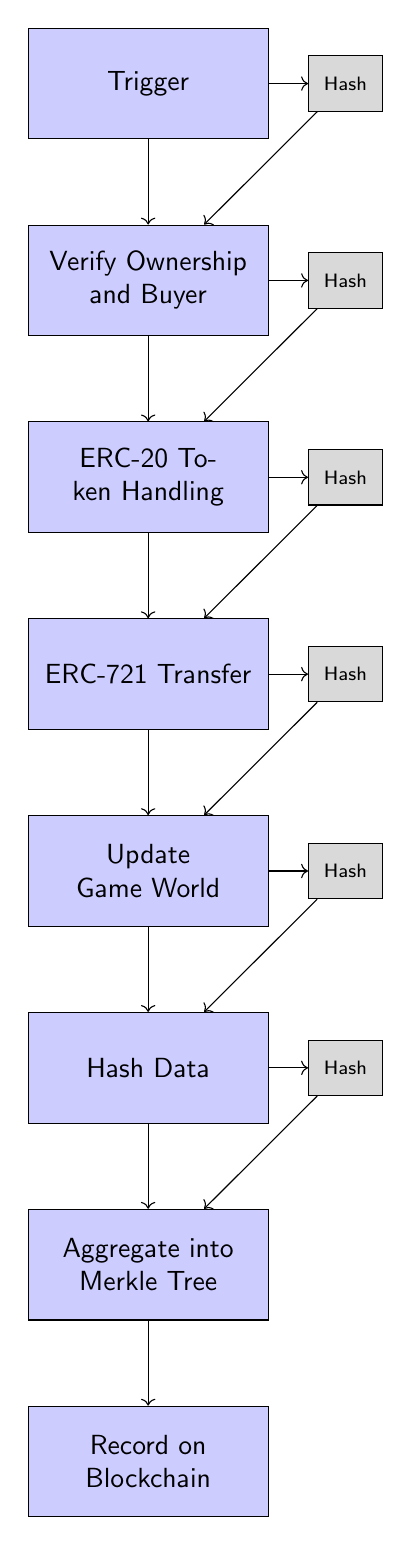
\begin{tikzpicture}[
    node distance=2.5cm and 2cm,
    auto,
    process/.style={rectangle, draw, fill=blue!20, text width=8em, text centered, minimum height=4em},
    mini process/.style={rectangle, draw, fill=gray!30, text width=2em, text centered, minimum height=2em, font=\scriptsize}
]
    % Main process nodes
    \node (trigger) [process] {Trigger};
    \node (verify) [process, below of=trigger] {Verify Ownership and Buyer};
    \node (erc20) [process, below of=verify] {ERC-20 Token Handling};
    \node (erc721) [process, below of=erc20] {ERC-721 Transfer};
    \node (update) [process, below of=erc721] {Update Game World};
    \node (hash) [process, below of=update] {Hash Data};
    \node (merkle) [process, below of=hash] {Aggregate into Merkle Tree};
    \node (blockchain) [process, below of=merkle] {Record on Blockchain};

    % Mini hash nodes to show data flow
    \node (mini0) [mini process, right=0.5cm of trigger] {Hash};
    \node (mini1) [mini process, right=0.5cm of verify] {Hash};
    \node (mini2) [mini process, right=0.5cm of erc20] {Hash};
    \node (mini3) [mini process, right=0.5cm of erc721] {Hash};
    \node (mini4) [mini process, right=0.5cm of update] {Hash};
    \node (mini5) [mini process, right=0.5cm of hash] {Hash};

    % Paths
    \draw[->] (trigger) -- (verify);
    \draw[->] (verify) -- (erc20);
    \draw[->] (erc20) -- (erc721);
    \draw[->] (erc721) -- (update);
    \draw[->] (update) -- (hash);
    \draw[->] (hash) -- (merkle);
    \draw[->] (merkle) -- (blockchain);

    % Mini hash paths
    \draw[->] (trigger) -- (mini0);
    \draw[->] (mini0) -- (verify);
    \draw[->] (verify) -- (mini1);
    \draw[->] (mini1) -- (erc20);
    \draw[->] (erc20) -- (mini2);
    \draw[->] (mini2) -- (erc721);
    \draw[->] (erc721) -- (mini3);
    \draw[->] (mini3) -- (update);
    \draw[->] (update) -- (mini4);
    \draw[->] (mini4) -- (hash);
    \draw[->] (hash) -- (mini5);
    \draw[->] (mini5) -- (merkle);
\end{tikzpicture}
\caption{Verifiability Process in W3.io Network}
\label{fig:verifiability_process}
\end{figure}


Upon the completion of a recipe, the final hash, along with the hashes of other concurrently completing recipes, is aggregated into a Merkel tree. This tree is structured based on specific criteria such as time or the count of recipe runs. The root of this Merkel tree is then recorded on the customer's preferred blockchain or on the default W3.io blockchain. This Merkel root serves as a verifiable record that can be used to confirm the integrity of any individual recipe execution.

Furthermore, the logged data is stored by default on IPFS (InterPlanetary File System), provided by Protocol Labs, one of our network partners. Customers also have the option to store their data on other long-term storage solutions such as Arweave or Space \& Time, depending on their specific requirements.

This comprehensive approach to verifiability not only ensures that each recipe runs as intended but also allows customers to verify the results for as long as the logs are maintained. For perpetual verification, customers can opt for permanent storage solutions. The trust assumptions of our partners are also considered and integrated into the metadata of each operation, ensuring that all aspects of the execution are transparent and verifiable.

\subsubsection{Consensus}
The W3.io network employs a flexible consensus mechanism, allowing for the adaptation of various consensus algorithms based on the specific needs of each recipe. This flexibility is crucial as it enables the network to operate efficiently without being bound to a single consensus method, which can often be costly and less adaptable.

We support several notable consensus mechanisms, each chosen for its unique benefits depending on the operational requirements:
\begin{itemize}
    \item \textbf{Tendermint:} Combines the speed of consensus algorithms like PBFT with the decentralized nature of blockchain. It is well-suited for blockchain services that require high performance and fast finality. Tendermint is particularly effective in environments where participants are known and reliability is required \parencite{kwon2014tendermint}.
    \item \textbf{Practical Byzantine Fault Tolerance (PBFT):} Designed to work well in asynchronous systems, PBFT can provide high throughput and low latency, making it ideal for distributed networks that need to achieve consensus even in the presence of faulty or malicious nodes \parencite{castro1999practical}.
    \item \textbf{Hedera Hashgraph:} Known for its high throughput and fast finality, Hedera is ideal for applications requiring quick transaction processing \parencite{baird2016swirlds}.
    \item \textbf{Stellar Consensus Protocol (SCP):} Offers low latency and flexible trust, suitable for low-cost and efficient consensus without requiring intensive proof-of-work \parencite{mazieres2015stellar}.
\end{itemize}

Nodes participating in a recipe's consensus are selected by the decentralized task queue and work collaboratively to reach consensus at each step of the recipe. This includes both read and write operations:
\begin{itemize}
    \item \textbf{Write Operations:} Require consensus before execution; the decentralized task queue then directs the write to an appropriate executor with the signed consensus of the nodes.
    \item \textbf{Read Operations:} All reads must be validated by consensus. Special considerations are made for operations like proof of inference, where reads may not be identical but still need to be verified.
\end{itemize}

The choice of consensus mechanism can significantly impact the performance and cost-effectiveness of a recipe. For example, a cost-sensitive customer might opt for Stellar's SCP for its efficiency, while a security-focused customer may prefer Ethereum's robust Proof of Work system. Ultimately, W3.io's flexible consensus approach ensures that the results of any recipe or ingredient run are verifiably correct and then verifiably recorded.

\subsubsection{Trusted Execution Environments (TEEs)}
Trusted Execution Environments (TEEs) are utilized within certain nodes of the W3.io network to enhance security and provide fully automated transaction signing. These environments provide an isolated execution space that protects sensitive computations from external threats, including those from the host machine. Nodes equipped with TEEs are incentivized to perform sensitive or critical tasks, ensuring robust security measures are in place for operations that require higher trust levels.

We collaborate with partners like Cubist, Lit Protocol, etc, which specialize in providing solutions along these lines. These partnerships are part of our roadmap towards a fully decentralized offering. Over time, we aim to integrate more decentralized TEE solutions to align with our vision of a fully decentralized network capable of permissioned execution on our customers behalf within their complex business processes. This strategic approach allows us to leverage advanced security technologies while working towards greater decentralization.

\subsection{Protocol Services}

\needs{Audie to write}

\subsubsection{API}

\needs{Audie to write}

\subsubsection{UI}
\needs{Audie to write}

\subsubsection{Decentralized Task Queue}
\needs{Audie to write}

\section{Token Model (Light Overview)}
\needs{BEN AND AUDIE TO WRITE} 

\section{Business Model}
\needs{DAVID AND AUDIE TO WRITE}

\section{Conclusion}
The conclusion

\newpage
\printbibliography[heading=bibintoc, title={References}]

\appendix
\newpage
\section{Network Partners}
\begin{figure}[h]
    \centering
    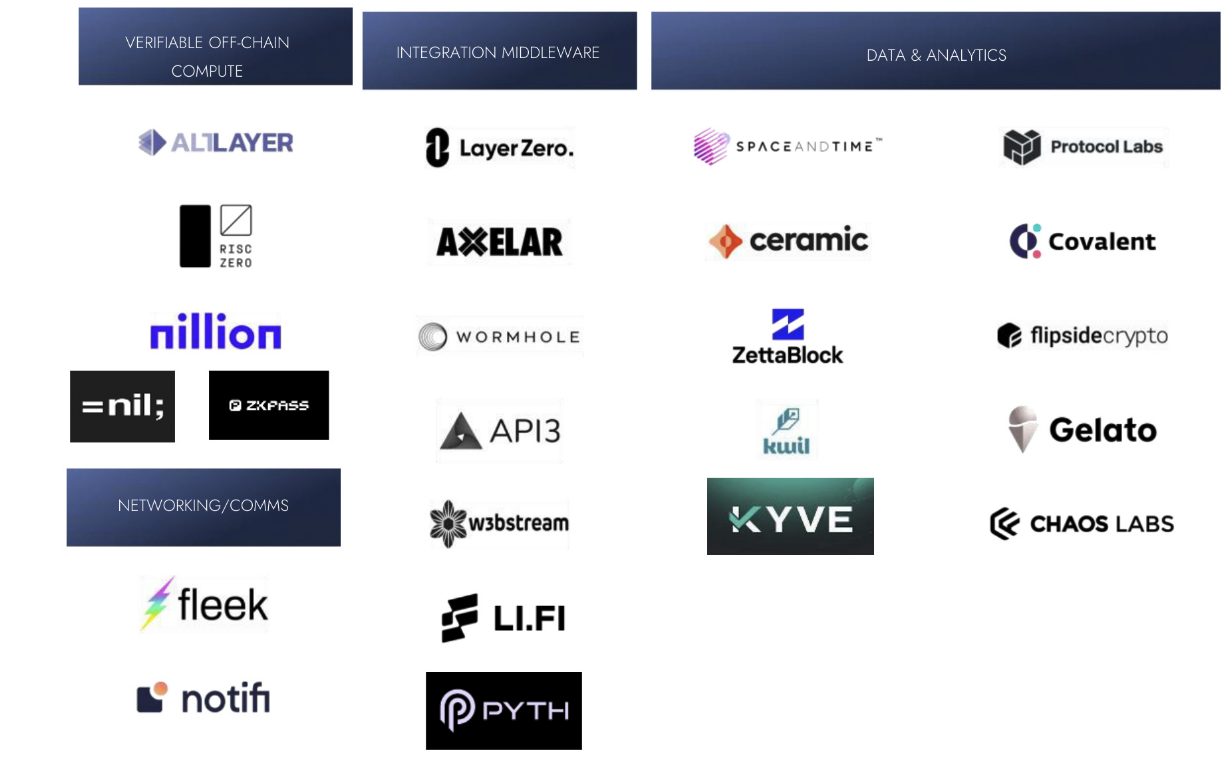
\includegraphics[width=0.75\textwidth]{images/Partners1.png}
    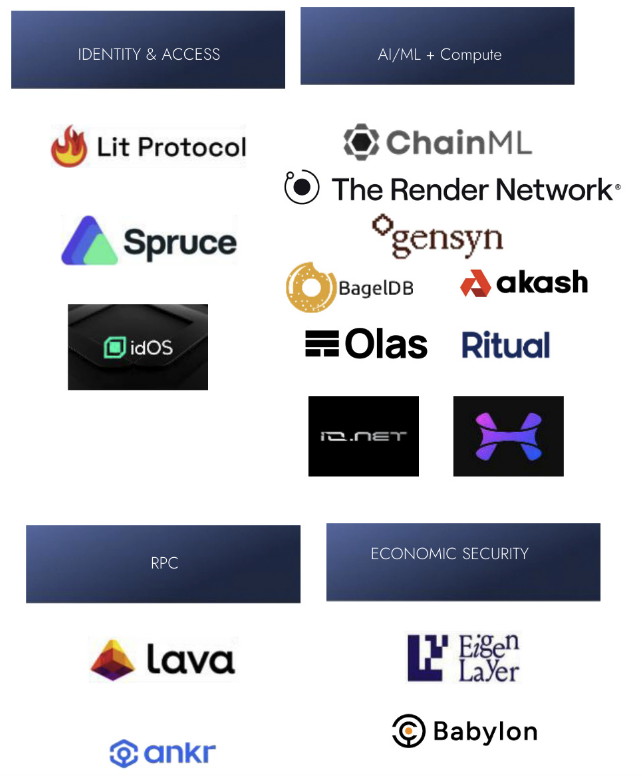
\includegraphics[width=0.4\textwidth]{images/Partners2.png}
    \caption{Network Partners}
    \label{fig:network-partners-appendix}
\end{figure}

\needs{Graphic Designer To Fix}

\newpage
\section{Team Profiles}
\needs{Graphic Designer and Marketing}

\newpage
\section{Appendix C: Mathematical Models}

\subsection*{Mathematical Model for Task Distribution in a Decentralized Network}
In this section, we develop a mathematical model to describe the distribution of tasks across a decentralized network. The model aims to ensure a fair and efficient allocation of tasks to various nodes within the network, leveraging cryptographic hash functions to achieve randomness and uniformity in task assignment. This approach not only enhances the security of the task distribution process but also ensures that no single node is overloaded, thereby maintaining the network's performance and reliability.

The model is designed to be scalable and adaptable, capable of handling varying numbers of nodes and tasks without significant changes to the underlying algorithm. This flexibility is crucial for the dynamic environment of decentralized networks, where the number of participating nodes and the volume of tasks can fluctuate significantly.

By mathematically modeling the task distribution, we provide a robust framework that supports the decentralized nature of the network and aligns with the principles of fairness and efficiency that are critical to the success of decentralized systems.

\subsection*{Variables}
\begin{itemize}
    \item \( N \): Total number of nodes in the network.
    \item \( R \): Total number of recipes that need to be executed.
    \item \( C \): Consensus group size required for each recipe.
    \item \( i \): Index of the current recipe.
    \item \( S_i \): Set of nodes selected for recipe \( i \).
    \item \( \text{hash}(x) \): A cryptographic hash function.
\end{itemize}

\subsubsection*{Process}
\begin{enumerate}
    \item \textbf{Initial Selection}:
    \[
    S_1 = \{ \text{hash}(1) \mod N, \text{hash}(2) \mod N, \ldots, \text{hash}(C) \mod N \}
    \]
    Ensure uniqueness in \( S_1 \) by rehashing if necessary.

    \item \textbf{Subsequent Selections}:
    \[
    S_i = \{ \text{hash}(S_{i-1}[1] \oplus i) \mod N, \ldots, \text{hash}(S_{i-1}[C] \oplus i) \mod N \}
    \]
    \( \oplus \) denotes a bitwise XOR operation.

    \item \textbf{Validation}:
    \[
    \text{hash}(\text{hash}(S_{i-1}[j] \oplus i) \oplus j) \mod N
    \]
    Check for node repetition and recompute if necessary.
\end{enumerate}

\subsubsection*{Justification}
\begin{itemize}
    \item \textbf{Uniformity}: The hash function ensures uniform distribution of node indices.
    \item \textbf{Memory}: Incorporating \( S_{i-1} \) prevents the same nodes from being selected repeatedly.
    \item \textbf{Scalability}: The method scales linearly with the number of nodes and recipes.
\end{itemize}

\end{document}

\end{document}